% -*- coding: utf-8; mode: latex; -*-

% +++
% latex = "lualatex"
% +++

%
% FIT2023 向け LaTeX クラスファイル
% https://github.com/trueroad/FITpaper-class
%
% サンプルファイル
%
% Copyright (C) 2018, 2019, 2022, 2023 Masamichi Hosoda.
% All rights reserved.
%

\documentclass{FITpaper}

% 図の貼り込み用
\usepackage{graphicx}
\usepackage{url}
\usepackage{comment} 
% 最終ページで両カラムの下端を揃える
%\usepackage[balance]{nidanfloat}
\usepackage{flushend}
\def\BibTeX{{\rm B\kern-.05em{\sc i\kern-.025em b}\kern-.08em
    T\kern-.1667em\lower.7ex\hbox{E}\kern-.125emX}}
% 和文タイトル
\jtitle{ブラウザ上でユーザが編集可能な言語パターンマッチシステムの構築 }

% 欧文タイトル
\etitle{Building a User-Editable Language Pattern Matching System in the Browser}

% 著者数:著者の数だけ c を書く
\authors{cc}

% 和文著者名:著者名間に & を書く
% 所属番号を \affmark でつける
\jauthors{%
  桂 辰弥\affmark{1} &
  竹内 孔一\affmark{2}
}

% 欧文著者名:著者名間に & を書く
\eauthors{%
  Tatsuya Katsura &
  Koichi Takeuchi
}

% 所属
% \affmark でつけた番号毎に指定
\afftext{1}{岡山大学大学院環境生命自然科学研究科\hskip1em
Graduate School of Environmental, Life, Natural Science and Technology, 
Okayama University}
\afftext{2}{岡山大学学術研究院\hskip1em
Academic Research Assembly,
Okayama University}

\begin{document}

\maketitle

\section{はじめに}
テキスト中の特定のフレーズや表現を見つけることは,言語および教育分野において必要となることがある.
テキストデータから特定のキーワードやフレーズの出現位置や文脈を抽出するためのプログラムとしてコンコーダンサがある.
テキストコーパス内の文字列や単語を検索し,検索単語を中心として,前後の文脈とともに示されるKWIC形式のように表示するコンコーダンサは既に数多く存在し\cite{WebParaNews:2014}\cite{corpusworkshop:2012},
これらを用いることで語彙や文法の理解,単語の使用法や文脈の把握に役立ち,学習者の語彙や表現力の向上に役立つ.
パターンマッチングはテキストの表層で検索を行う正規表現とは異なり,情報を抽出したい文を対象に予め関係する文や文の一部に対応する文構造のパターンを用意し,そのパターンに合致する結果を取得するものである.
有名なコンコーダンサの例として,Sketch Engineがある.Sketch Engine\footnote{https://www.sketchengine.eu/},はクエリ言語としてCQL\footnote{https://www.sketchengine.eu/documentation/corpus-querying/}が使用されており,正規表現を用いて複雑な条件やパターンに基づいたデータの検索や抽出が可能である.
他にもStruAP\cite{struAP:2017}があり,係り受り構造を利用し、部分木パターンによる関係抽出ができるツールである.
しかしこれらのコンコーダンサやパターンマッチを行えるツールの多くは商用ツールであるため,利用しにくい.
言語解析者や語学学習者が文構造を考慮してテキスト中の特定フレーズや表現を抽出するようなシステムを構築することは容易ではない.そこで本研究では解析モジュールで解析した結果をユーザ自身が求める表現をあらかじめ用意された検索ブロックで組み合わせてシステムに投入し,事例を検索できるシステムの開発を行っている.先行研究\cite{okada2021}\cite{ogasawara2021}においてWEBアプリケーションとしてJavaScriptとPythonを利用した基本システムを構築したが,
システムの本格利用にはいくつかの課題が残されている.そこで本報告では検索エンジンの中心部分であるPrologデータベースの実装の改良,および,大規模なテキストが扱えるためにデータベースをシステムに導入したので,この改良について報告する.


\section{提案するパターンマッチシステムの概要}
本章では開発したパターンマッチシステムを構築する環境と実際のシステムの処理の流れについて述べる.
%また先行研究との大きな変更点であるPrologデータベースの実装の改良,および,大規模なテキストが扱えるためにデータベースをシステムに導入についても触れている.

\subsection{提案するパターンマッチシステムの構成}

\begin{figure}[htbp]
  \centering
  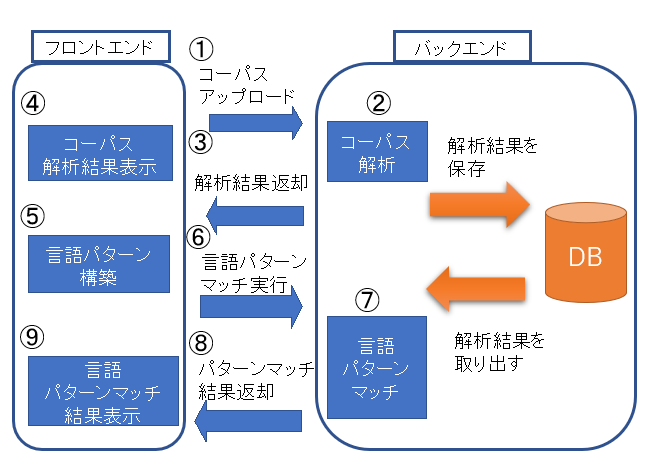
\includegraphics[scale=0.4]{fig/system_fig.png}
  \caption{システムの構成図}
  \label{fig:sys}
\end{figure}

本システムは図\ref{fig:sys}のようにユーザが視覚的に操作を行うフロントエンドシステムとユーザが要求したテキストの処理バックエンドシステムに切り分けて構成している.
フロントエンドシステムはJavaScriptのライブラリであるReactで構成されており
主な機能としてはテキストファイルのアップロード,検索する言語パターンの構築,解析結果の表示,検索結果の表示などがある.
バックエンドシステムはPythonのWebフレームワークであるDjangoとデータベースシステムであるElasticsearch\footnote{https://www.elastic.co/jp/elasticsearch/}で構成されており,
主な機能としてはテキストファイルの解析,検索クエリの言語パターンマッチ実行などがある.
詳しい処理の流れについては以降の節で述べる.

\subsection{バックエンドの処理の流れについて}
バックエンドの処理の流れとしてテキスト解析,言語パターンマッチ実行の処理についてそれぞれ説明する.

\begin{figure}[htbp]
  \centering
  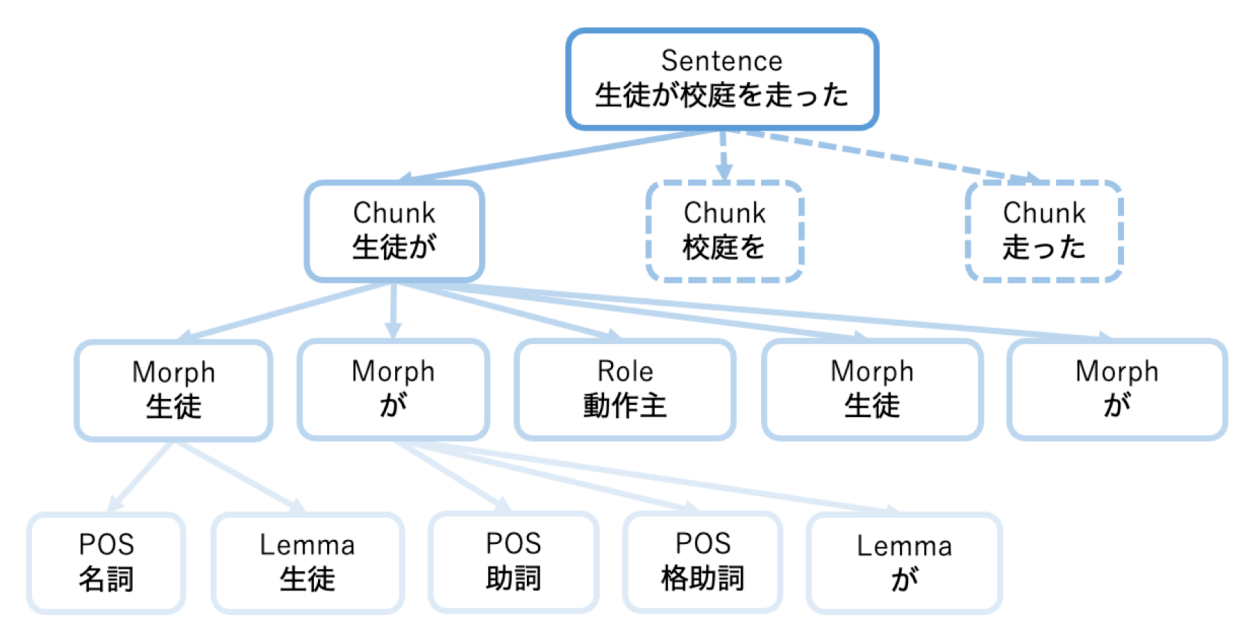
\includegraphics[scale=0.4]{fig/tree.eps}
  \caption{文を解析した木構造の例}
  \label{fig:tree}
\end{figure}
\begin{table}[htbp]
  \caption{Prologの述語一覧}
  {\footnotesize
  \begin{center}
    \begin{tabular}{|l|l|l|l|}\hline
      述語                    &第1引数     &  第2引数   & 第3引数               \\
      \hline 

      chunk(\_, 0,\_)       &文番号    &  0固定& 文節 ID                   \\
      morph(\_, \_, \_)     &文番号 & 文節 ID& 形態素 ID                \\
      main(\_, \_, \_)      &文番号   &文節 ID & 主形態素 \\
      part(\_, \_, \_)      &文番号   &文節 ID& 副形態素\\
      role(\_, \_, \_)      &文番号   &文節 ID& 意味役割  \\
      semantic(\_, \_, \_)   &文番号  &文節 ID & 概念\\
      surf(\_, \_, \_)        &文番号  &ノード ID& 表層\\               
      surfBF(\_, \_, \_)      &文番号 &形態素 ID& 基本形        \\
      sloc(\_, \_, \_)  &文番号&文節/形態素 ID & 文中出現位置\\
      pos(\_, \_, \_)    &文番号      &形態素 ID& 品詞\\                                        
      dep(\_, \_, \_)     &文番号   &文節 ID & 係り受け文節 ID\\
        \hline
    \end{tabular}
  
    \label{tbl:predicates}
  \end{center}
  }
\end{table}



テキスト解析の処理はユーザがテキストファイルのアップロードを行うことで実行される.
送られたテキストファイルの文にASA\footnote{https://github.com/Takeuchi-Lab-LM/python\_asa/}を用いて形態素解析と項構造を適応させる.解析した結果の文の木構造を図\ref{fig:tree}に示す.
その後Prolog述語に変換を行い,データベースに保存する.データベースに保存する際には,1文ごとに対応した解析データを保存している.
変換するProlog述語は以下の表\ref{tbl:predicates}のように定義している.%図\ref{fig:prolog}のように変換される.
ASAで解析したデータがJSON形式であるため,Elasticsearchをデータベースとして活用することで,
JSON形式の大規模な解析データの柔軟な取り扱いや高速な検索,リアルタイムな更新,スケーラビリティ,高度な分析など,データベースとしての利点を最大限に生かすことができる.
言語パターンマッチの処理はフロントエンドからユーザが構築した言語パターンが送られると,データベースから各文に対応するPrologデータを取得し,
1文ずつPrologデータと検索クエリでパターンマッチを実行し,マッチ解の生成を行う.
パターンマッチを実行するProlog処理系としてSWI-PrologのPythonモジュールであるpyswipを使用している.
Prolog処理系として採用したSWI-Prolog\footnote{https://www.swi-prolog.org/}はCで記述された高機能のProlog処理系であり,
SWI-Prologの強力な論理プログラミング機能とPythonのデータ処理能力を組み合わせることで,高速でより拡張性の高い環境が提供される.







%\begin{figure}[htbp]
 % \centering
  %\includegraphics[scale=0.5]{fig/prolog_data.png}
  %\caption{変換されたprolog}
  %\label{fig:prolog}
%\end{figure}


\subsection{フロントエンドの表示機能について}
次にフロントエンドでの解析結果,検索クエリとなる言語パターンの構築,検索結果の表示について説明する.
\begin{figure}[htbp]
  \centering
  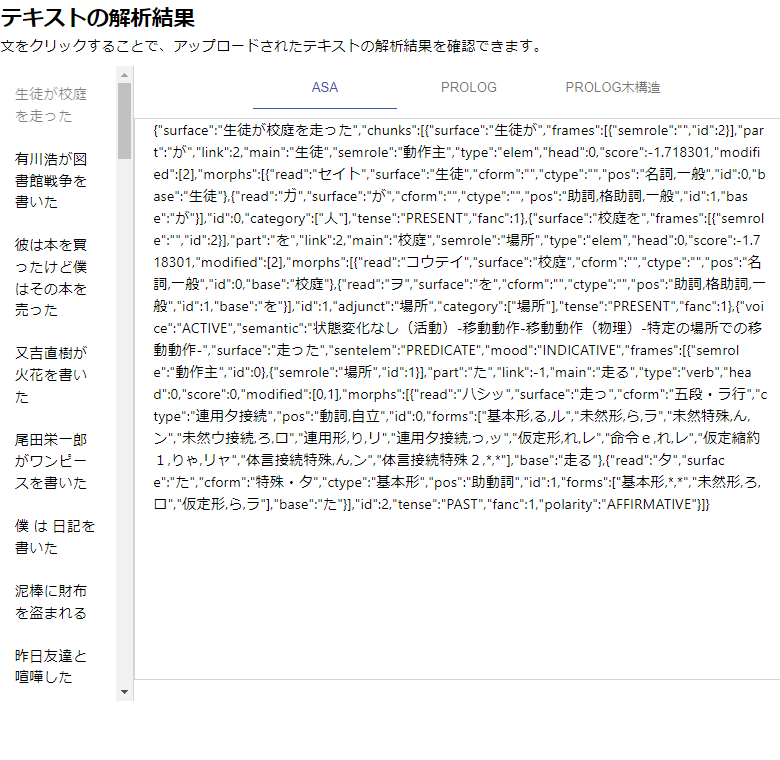
\includegraphics[scale=0.4]{fig/convert_result_asa.png}
  \caption{解析結果の例(ASA)}
  \label{fig:show_ASA}
\end{figure}
\begin{figure}[htbp]
  \centering
  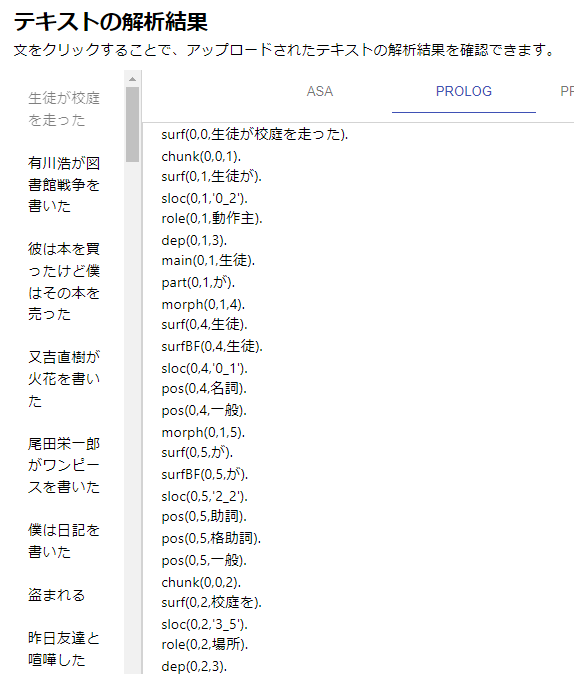
\includegraphics[scale=0.4]{fig/convert_result_prolog.png}
  \caption{解析結果の例(Prolog)}
  \label{fig:show_prolog}
\end{figure}

フロントエンドはテキスト解析の処理終了後,解析結果をデータベースから取得して表示する.以下の図\ref{fig:show_ASA},\ref{fig:show_prolog}は解析結果の表示例である.
1文ごとに対応した解析データを保存するようにデータベースに保存しているので,
解析データの表示の際には文をクリックするたびにその文に対応する解析データを取得するように実装している.


\begin{figure}[htbp]
  \centering
  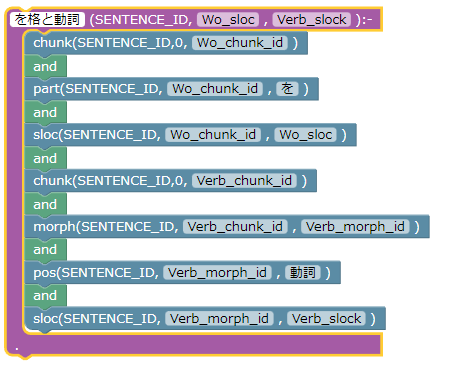
\includegraphics[scale=0.6]{fig/wo.png}
  \caption{「ヲ格と動詞」の言語パターン}
  \label{fig:wo_block}
\end{figure}

\begin{figure}[htbp]
  \centering
  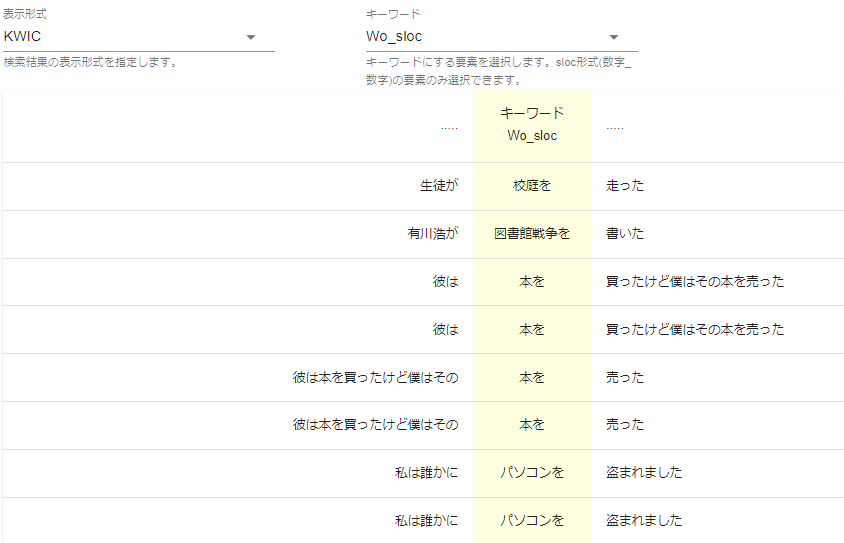
\includegraphics[scale=0.3]{fig/KWIC_result.png}
  \caption{KWIC表示}
  \label{fig:KWIC}
\end{figure}
\begin{figure}[htbp]
  \centering
  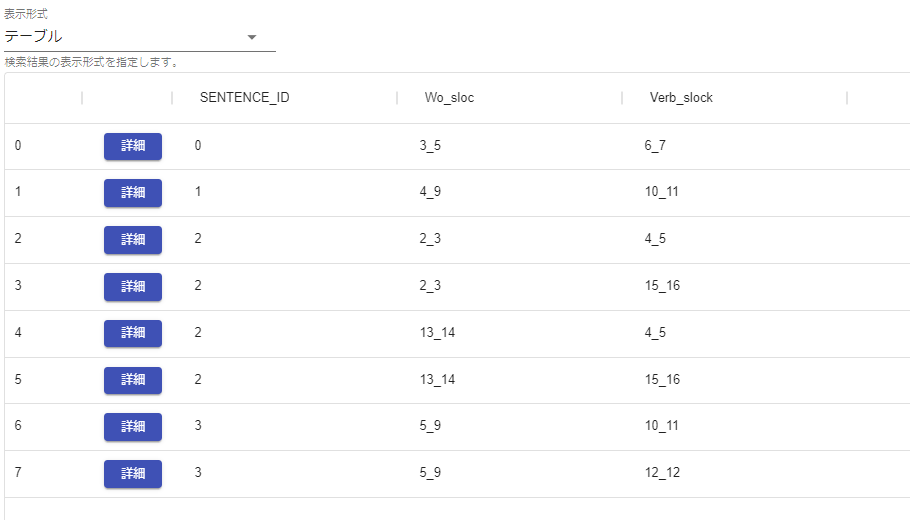
\includegraphics[scale=0.3]{fig/table_result.png}
  \caption{テーブル表示}
  \label{fig:table}
\end{figure}
\begin{figure}[htbp]
  \centering
  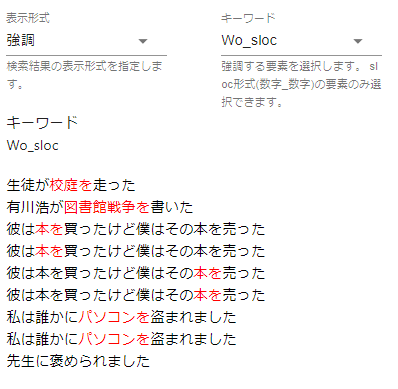
\includegraphics[scale=0.4]{fig/acsent_result.png}
  \caption{強調表示}
  \label{fig:acsent}
\end{figure}





言語パターンを構築するにはBlockly\footnote{https://developers.google.com/blockly?hl=ja}で定義されたブロックを利用する.
前節で示したProlog述語のブロックをユーザが自ら組み合わせることで,複雑な検索クエリを構築することができる.
図\ref{fig:wo_block}に例を示す.パターンマッチを実行するとバックエンドから検索結果を受け取り,結果を表示する.表示の際にはKWIC,テーブル,強調の3つの表示形式を選択することができる.
以下の図\ref{fig:KWIC},\ref{fig:table},\ref{fig:acsent}は図\ref{fig:wo_block}の検索結果の表示例である.
引数\textit{Wo\_Slock},\textit{Verb\_Slock}は文中での出現位置を示しており,検索パターンの引数に\textit{\_Slock}を含む場合と表示形式で強調する要素を選択できるようになる.
図\ref{fig:KWIC}は「ヲ格」,図\ref{fig:acsent}は「動詞」の要素を強調して表示することで視覚的にわかりやすくしている.


\section{動作評価実験}
システムの動作評価実験を行い,パターンマッチシステムの処理性能の向上の確認を行う.

\subsection{実験内容}
\begin{table}[htbp]
  \centering
    \caption{ファイルサイズ(バイト)}
    \label{tbl:txt}
    \begin{tabular}{|r||r|}  
      \hline
      文の数 & ファイルサイズ\\ \hline \hline
      1 & 46\\\hline
      10 & 440 \\\hline
      100 & 5,342\\ \hline
      1000 & 53,248 \\\hline
      5000 &  262,199 \\\hline
      10000 &  524,399\\ \hline
    \end{tabular}
  \end{table}

表\ref{tbl:txt}に示すテキストファイルを用意し,
テキスト解析とパターンマッチを行い,これらの処理時間を先行研究のシステムと提案するパターンマッチシステムでそれぞれ計測した.
具体的にはフロントエンドからバックエンドに送信し,バックエンドからデータが返ってくるまでを処理時間として計測する.
これらの処理時間はChromeのデベロッパーツールを用いて計測を行う.
検索クエリは表\ref{fig:wo_block}の「ヲ格と動詞」の言語パターンを用いる.


\subsection{実験結果}

\begin{table}[htbp]
  \centering
    \caption{テキスト解析の処理時間(秒)}
    \label{tbl:convert_time}
    \begin{tabular}{|r||r|r|}  
      \hline
      文の数 &先行研究のシステム& 提案するシステム \\\hline \hline
      1 & 0.083&0.144\\\hline
      10 & 0.414&0.453 \\\hline
      100 & 3.50 &3.56\\ \hline
      1000 & 35.3&36.4 \\\hline
      5000 &  174&192\\\hline
      10000 &  計測不能&768\\ \hline
    \end{tabular}
  \end{table}
\begin{table}[htbp]
  \centering
    \caption{パターンマッチの処理時間(秒)}
    \label{tbl:matching_time}
    \begin{tabular}{|r||r|r|}  
      \hline
      文の数 & 先行研究のシステム& 提案するシステム\\ \hline \hline
      1 & 0.110&0.242\\\hline
      10 & 0.440 &0.495\\\hline
      100 & 8.15&1.65\\ \hline
      1000 & 960 &30.9 \\\hline
      5000 & 計測不能 &78.4\\\hline
      10000 & 計測不能 &160\\ \hline
    \end{tabular}
  \end{table}


  パターンマッチの動作評価実験の結果をそれぞれ表\ref{tbl:convert_time},\ref{tbl:matching_time} に示す.
  テキスト解析,パターンマッチ実行はともに文の数が増えるにつれ,処理時間も増加していることが読み取れる.

  
  テキスト解析の処理時間については
  先行研究のシステムは10000 文のテキストファイルを処理する際には動作が止まってしまったが,提案するシステムでは10000文でも動作が確認できた.
  提案するパターンマッチシステムはは先行研究のシステムに比べ,処理時間が少し大きくなっているが微差である.
 
  パターンマッチシステムの処理時間については
  先行研究のシステムは
  5000 文のテキストファイルを処理する際には動作が止まってしまったが,提案するシステムでは10000文でも動作が確認できた.
  提案するシステムは10000文のテキスト解析,パターンマッチ実行がともに動作を確認できた.
  また100文以上のパターンマッチの処理時間が向上しており,
  全体的にシステムの処理性能の向上が確認できた.
  
  ただし10000文の処理を行った際にはブラウザの挙動が重くなるため,ユーザの操作に対する影響という新たな課題を確認した.
  
\section{考察}
  テキスト解析の処理時間は先行研究のシステムに比べ,少し遅くなったが,これはデータベースを1文ごとに対応した解析データを保存するように改良を行ったためであり,
  10000文を解析を行った際には10000個の解析データを保存する必要があるため,バックエンドにおけるDjangoとデータベースシステムとのやりとりの時間が増加してしたためである.
  今回の実装では1文ずつPrologデータベースに追加し,パターンマッチを生成した.
  実際には全文で解探索するほうが,処理時間が小さくなるが,全文のPrologデータの記述されたファイルの生成に多くの時間がかかるため,
  1文ずつPrologデータベースに追加する実装に変更した.
  しかしこの実装の問題点として,例えば10000文のパターンマッチを行う際には10000回処理を行うPrologファイルの生成を行う必要があり,バックエンドシステムへの負荷が大きい,
  そのためファイル生成を行わずにパターンマッチを実行する実装方法を検討する必要がある.
  Elasticsearchは、1度に取得することができるドキュメントの最大件数は、デフォルトでは10,000件であるためであり,
  10000文以上のテキストファイルの解析は現状の手順では対応できない.
  また提案するパターンマッチシステムは10000文まで解析やパターンマッチが可能となったが,さらに解析後のブラウザの挙動がかなり重くなっており,
  ユーザが利用可能とは言い難い.
  今後さらに処理性能の向上させるには,パフォーマンスの問題やネットワークの制約などに留意して実装する必要がある.
  

  現在の実装では,柔軟なパターンマッチを行うためには,ユーザがPrologに精通している必要がある.
  より簡単な操作を実現する方法としては表層に"*"のような曖昧性を含んだ正規表現を持つクエリとPrologのパターンマッチの実装が考えられる.今回 Prolog 処理
系として導入した SWI-Prolog は正規表現に対応可能な regex パッケージが存在するため,今後の課題として正規表現マッチのシステムの導入が考えられる.

\section{まとめ}
  本研究では,先行研究のシステムをベースに開発を進め,
  検索エンジンの中心部分であるPrologデータベースの実装の改良として,Prolog処理系としてSWI-Prologを導入し,
  1文ずつPrologデータと検索クエリでパターンマッチを実行し,マッチした解を生成するように実装した.
  また,大規模なテキストを扱うためにデータベースとしてElasticsearchをシステムに導入した.
  実装した機能の処理性能を確認するための動作評価実験を行い,10000文のテキストの動作することを確認した.
  今後の課題としてさらなる処理性能の向上と正規表現マッチの追加が考えられる.



\acknowledgment{%
本研究の一部は、日本学術振興会科学研究費補助金(助成番号22K00530)の助成を受けた.
%本研究の一部はJSPS科研費JP22k00530の助成を受けた.
}


\bibliography{biblio.bib}
\bibliographystyle{junsrt}
%\bibliographystyle{unsrt}

%\bibliography{all,my-results}

\end{document}
